\documentclass[12pt,t]{beamer}
\usetheme[greyauthor, % Grå tekst forfatter som KU vil have
         unit=NAT, % Ændre til NAT, KU, eller unit=ics (diku)
         dk, % Sprog
         %style=simple, % Vandmærke eller billede
         footstyle=low, % Fjern stor footer
         wmark, % vandmærke på hver side
         logoplace=left % Logo til venstre
         %,sidebar % makes sidebar
         ]{Frederiksberg}
% nat for Science, ku for generic or unit=ics for DIKU
% Tilføj style=simple for vandmærke
\usepackage{listings} % Pakke til kode
\usepackage{pslatex}        % pæn skrift
\usepackage[utf8]{inputenc} % Implementerer Unicode
\usepackage{algpseudocode}
\usepackage{algorithm}
\usepackage{color}
\usepackage{minted}

\title{Espergærde Gymnasium}
\subtitle{Algoritmer og problemløsning}
\author{
        Gymnasietjenesten på DIKU
}

\date[]{\today}


\begin{document}

\frame[plain]{\titlepage}

\section{Dagens program}

\begin{frame}
    \frametitle{Program for idag}
    \begin{block}{Indtil kl 11.30}
        \begin{itemize}
            \item Algoritme design og metoder. \pause
            \item Hvordan man kan sammenligne forskellige løsninger. \pause
            \item Intro til iPython \pause
            \item Intro til Machine Learning \pause
        \end{itemize}
    \end{block}
    \pause
    \begin{block}{Fra 12.00 til 13.30}
        \begin{itemize}
            \item Perceptron \pause
            \item K-means Clustering
        \end{itemize}
    \end{block}
    \begin{block}{Fra 13.45 til 15.00}
        \begin{itemize}
            \item Øvelser
        \end{itemize}
    \end{block}
\end{frame}


\section{Introduktion til algoritmer}
    \begin{frame}[c]{Hvad er en Algoritme?}
        \begin{quote}
            An algorithm is a self-contained step-by-step set of operations to
            be performed that can be expressed within a finite amount of space
            and time and in a well-defined formal language.
        \end{quote}
        \pause
        \begin{block}{På dansk}
            En algoritme er en \alert{opskrift} på hvordan et bestemt problem
            kan løses.
        \end{block}
    \end{frame}


    \begin{frame}[plain]{Havregryns algoritme}
        \begin{block}{Eksempel}
        \vspace{-1.5em}
        \begin{algorithm}[H]
            \caption{\newline Indgangsbetingelser: En skål, mælk, havregryn
                     \newline Udgangsbetingelser: Morgenmad
            }
            \begin{algorithmic}
                \While{Skålen ikke er fyldt}
                    \State Hæld Gryn i Skålen
                \EndWhile
                \If{Jeg er tyk}
                    \State mælk = Minimælk
                \Else
                    \State mælk = Letmælk
                \EndIf
                \While{Skålen ikke er fyldt}
                    \State Hæld mælk i Skålen
                \EndWhile
            \end{algorithmic}
        \end{algorithm}
        \end{block}
    \end{frame}

    \begin{frame}
        \frametitle{Krav til en algoritme?}
        \begin{block}{Krav til en algoritme}
        \begin{description}
            \item[Veldefineret] Ingen tvetydigheder og vendinger som:``
            så tager du det bedste resultat $\dots$'' \pause
            \item[Terminerer] Den må ikke køre for evigt, du skal garantere
            at den rent faktisk finder sit svar. \pause
            \item[input og output] Jeg skal vide at hvis jeg giver
            den $A$ så returnerer den $B$. \pause
            \item[Kan bevises] Det er muligt både at bevise korrekthed og
            køretid for algoritmen.
        \end{description}
        \end{block}
    \end{frame}

    \begin{frame}[t]{Eksempler på algoritmer}
        Algoritmer bruges inden for alle former for problemløsnings. \pause
        \begin{block}{Bioinformatik}
            \emph{Longest commen subsequence: } Sammenligning af DNA strenge
            for at se hvor beslægtet to strenge er. \pause
        \end{block}
        \begin{block}{Primtals faktorisering}
            Bruges i \emph{kryptering: } Basis for at vi kan have sikker
            kommunikation. \pause
        \end{block}

        \begin{block}{Machine Learning}
            En samling af algoritmer der selv kan lære og finde egenskaber
            i store data sæt. Gør det muligt at løse problemer der før var
            uden for menneskers kunnen.
        \end{block}
    \end{frame}


\section{Algoritme vs Algoritme}
    \begin{frame}[t]{Valget af algoritme}
        \begin{exampleblock}{Soterings algoritmer}
            Givet en liste af $n$ tal ønsker vi at returnere en sorteret liste
            af længde $n$.
        \end{exampleblock}
        \pause
        \vspace{-2em}
        \begin{columns}
            \begin{column}{0.5\textwidth}
                \begin{block}{Hold $A$}
                    \begin{itemize}
                        \onslide<+->{\item Har en computer}
                        \onslide<+->{\item Bruger algoritmen \emph{Merge Sort}}
                        \onslide<+->{\item De kan sortere $10$ millioner tal på
                                     under $20$ minutter}
                        \onslide<+->{\item De kan sortere $100$ millioner tal på
                                    $4$ timer.}
                    \end{itemize}
                \end{block}
            \end{column}
            \begin{column}{0.5\textwidth}
                \begin{block}{Hold $B$}
                    \begin{itemize}[<+->]
                    \item Har en computer der er $1000$ gange hurtigere end
                    hold A
                    \item Bruger algoritmen \emph{Insertion Sort}
                    \item De kan sortere $10$ millioner tal på $5$ timer.
                    \item De kan sortere $100$ millioner tal på \alert{23 dage!}
                    \end{itemize}
                \end{block}
            \end{column}
        \end{columns}
    \end{frame}

    \begin{frame}[t]{Sammenligning af Algoritmer}
        \begin{quote}
            Vi bruger begrebet \emph{Køretid} for at beskrive hvordan tiden en
            algoritme bruger stiger med input.
        \end{quote}
        \pause
        \vspace{-1em}
        \begin{block}{Definition på køretid}
            En øvregrænse for den tid der bliver brugt på at løse et problem af
            størelse $n$. Skrives som
            $$
                O(n), O(n^2), O(n \lg n), O(n!), O\left( \frac{a}{b} \right)
            $$
        \end{block}
        \pause
        \begin{exampleblock}{Algoritme for minimums funktionen}
            Givet en liste $X = [x_1,x_2,\dots,x_n]$ ønsker vi at returnere det
            mindste tal i listen. Hvad er algoritmen og hvad er køretiden?
        \end{exampleblock}
    \end{frame}

    \begin{frame}{Minimums algoritme}
        \begin{block}{Eksempel}
        \vspace{-1.5em}
        \begin{algorithm}[H]
            \caption{\newline Input: En liste $X=[x_1,x_2, \dots, x_n]$
                     \newline Ouput: Det mindste tal i listen.
            }
            \begin{algorithmic}
                \State min = $x_1$
                \For{$x_i$ in X}
                    \If{$x_i < \min$}
                        \State min = $x_i$
                    \EndIf
                \EndFor
            \end{algorithmic}
        \end{algorithm}
        \end{block}
        \pause
        \begin{block}{Analyse af algoritmen}
            \centering Køretid? \pause $O(n)$ \\
            \pause
            \centering Er den optimal? \pause \alert{Jeps!}
        \end{block}
    \end{frame}

    \begin{frame}[t]{Eksempler på køretid}
        \vspace{-2em}
        \begin{columns}
            \begin{column}{0.33\textwidth}
                \begin{block}{Bogo Sort}
                    \begin{itemize}
                        \item Køretid på $O(n!)$
                    \end{itemize}
                \end{block}
            \end{column}
            \begin{column}{0.33\textwidth}
                \begin{block}{Insertion Sort}
                    \begin{itemize}
                        \item Køretid? $O(n^2)$
                    \end{itemize}
                \end{block}
            \end{column}

            \begin{column}{0.33\textwidth}
                \begin{block}{Merge sort}
                    \begin{itemize}
                        \item Køretid på $O(n \lg n)$
                    \end{itemize}
                \end{block}
            \end{column}
        \end{columns}
        \begin{figure}[h!]
            \caption{Graf over køretider}
            \centering
            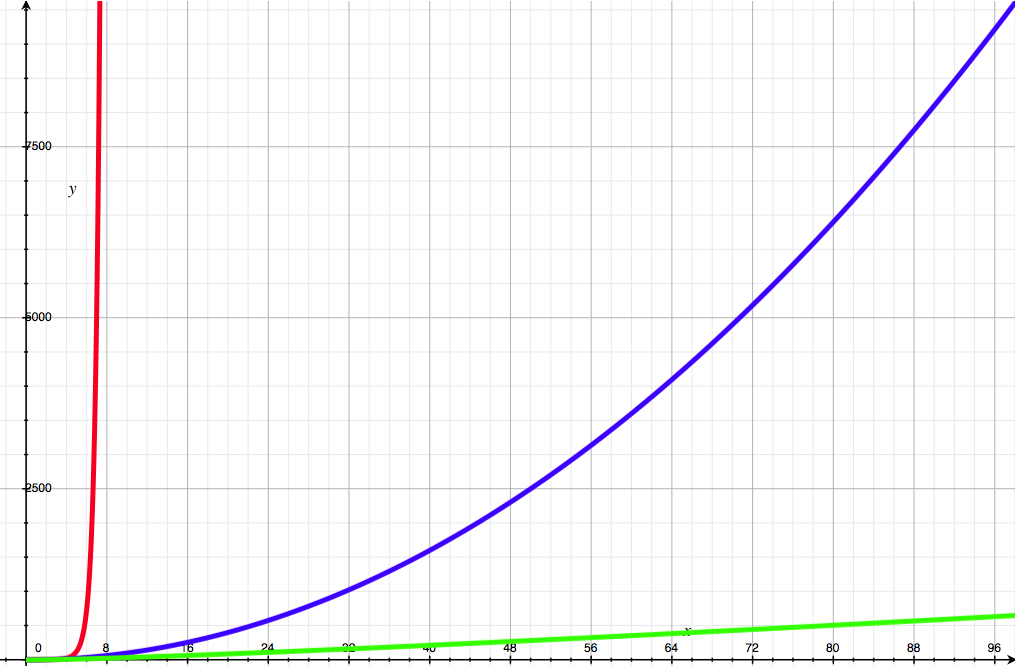
\includegraphics[width=0.7\textwidth]{./include/exs.png}
        \end{figure}
    \end{frame}


\section{Algoritme design}
    \begin{frame}[c]{Hvordan finder man på en algoritme}
        \begin{block}{Algoritme for algoritmer}
            \begin{enumerate}
                \item Beskriv problemet med egne ord. \pause
                \item Del problemet op i mindre dele. \pause
                \item Definer output \pause
                \item Definer input \pause
                \item Beskriv trin for at gå fra input til output
            \end{enumerate}
        \end{block}
    \end{frame}

    \section{Øvelser}
            \begin{frame}[t]{Øvelser}
                \begin{block}{Algoritme for øvelserne}
                    \begin{enumerate}
                        \item Der præsenteres et problem med eksempler. \pause
                        \item I finder på en algoritme for problemet
                              (Arbejd gerne sammen) \pause
                        \item Vi løser den sammen på tavlen. \pause
                    \end{enumerate}
                \end{block}
            \end{frame}

        \begin{frame}
          \frametitle{Søgning}
          \begin{block}{Mål}
          Givet en sorteret liste og et element, bestem om element er i listen,
          ved at kigge på så få elementer som muligt.
          \end{block}
          \pause

          \begin{exampleblock}{Eksempel}
          Lad en liste være givet ved $[2, 4, 5, 7, 8, 11, 25]$, hvor vi ønsker at
          finde ud af om elementet 11 er listen. Svaret skulle gerne være ja.
          (det første element har indeks 0).
          \end{exampleblock}
        \end{frame}

        \begin{frame}
          \frametitle{Sortering}
          \begin{block}{Mål}
              Sorter en givet usorteret liste.
          \end{block}
          \pause

          \begin{exampleblock}{Eksempel}
          Lad en liste være givet ved [7, 4, 5, 12, 1], denne vil vi gerne sortere!
          Den sorterede liste skulle gerne være [1, 4, 5, 7, 12].
          \end{exampleblock}
        \end{frame}

    \section{Fibonacci Tal}
        \begin{frame}[c]{Overlappende under problemer}
            \begin{block}{Eksempel}
                Det $n$'te\emph{Fibonacci} tal er defineret som summen af de to
                forgående.
                $$
                  1,1,2,3,5,8,13,21,34,55, \dots
                $$
                \pause
                Hvordan bestemmer vi dem?
            \end{block}
        \end{frame}


        \begin{frame}{Programmering}
                \begin{block}{Hvorfor skal vi kode?}
                    \begin{enumerate}
                        \item Vi kan bruge at computeren kan lave 10.240 millioner
                              instruktioner per sekund. \pause
                        \item Vi slipper for at håndkøre algoritmer \pause
                        \item Algoritmer kan testes og udføres med computere effektivt \pause
                        \item Vi kan arbejde med data som mennesker ikke kan overskue \pause
                        \item Computeren har allerede vist sig over menneskelig i visse
                        situationer.
                    \end{enumerate}
                \end{block}
            \end{frame}


         \section{Introduktion til python}
             \begin{frame}[t]{Hvorfor python?}
                 \begin{description}
                     \item[Høj niveaus sprog] Man skal ikke tænke på hvordan
                     maskinen fortolker det.
                     \pause
                     \item[Alsidigt] Bliver brugt mange steder,
                     fra webudvikling til kræftforskning
                     \pause
                     \item[Nemt at lære] Det har en simpel pæn syntax og er meget
                     tilgivende. Minder meget om pseudokode
                 \end{description}
                 \pause
                 \begin{block}{Minimums algoritmen}
                       \inputminted{python}{min.py}
                \end{block}
             \end{frame}

            \begin{frame}{Hvad med et gætte spil?}
                 Vi ønsker at kode et lille spil hvor brugeren skal gætte
                 det tal computeren har valgt.

                \begin{block}{Demo}
                    Den koder vi!
                \end{block}
            \end{frame}

            \section{Øvelser}
            \begin{frame}[t]{Øvelsestid}
                Kode øvelser i python!
            \end{frame}



\end{document}
